\chapter{Конструкторская часть}

\section{Общие сведения}

Положение объектов сцены в пространстве описывается с помощью
мировой системы координат, при этом ось Oz должна быть направлена вверх.

Общий алгоритм работы программы можно описать следующим образом:

\begin{enumerate}
	\item задать объекты сцены (камера, пол, источник света, слайм);
	\item для каждого кадра:
	\begin{enumerate}
		\item проверить характеристики объектов сцены;
		\item если пользователь пытается захватить фрагмент слайма, найти точки, входящие в область захвата, и запомнить их;
		\item определить силы, действующие на точки слайма;
		\item изменить скорости точек слайма в соответствии с действующими на них силами;
		\item переместить точки слайма, в соответствии с их скоростями.
		\item если пользователь захватил фрагмент слайма, переместить его в область пространства, соответствующую положению курсора мыши на экране;
		\item вывести изображение на экран.
	\end{enumerate}
\end{enumerate}

Моделируемый объект можно представить в виде множества точек, соединенных между собой пружинами. На рисунке \ref{slime_struct} приведена диаграмма структур данных, необходимых для хранения информации о слайме.

\begin{figure}[H]
	\centering
	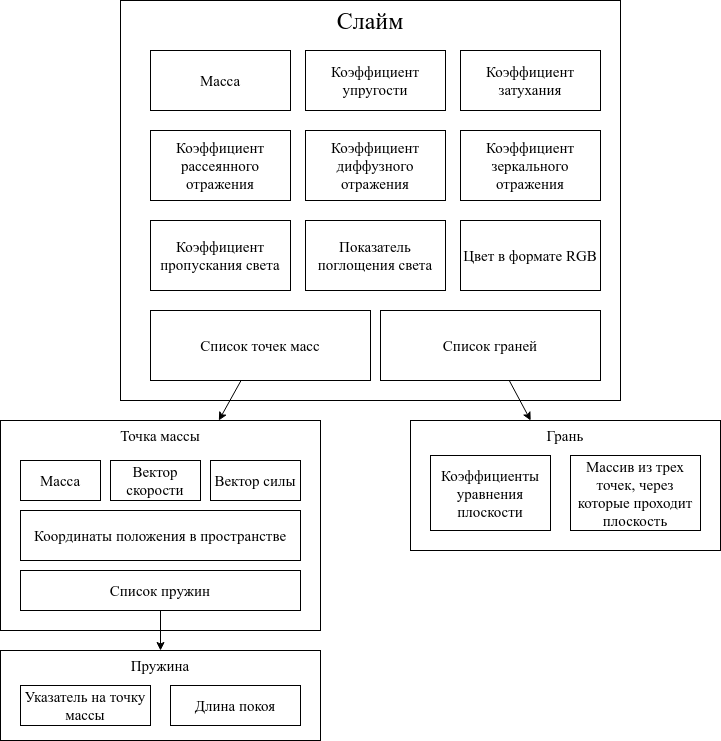
\includegraphics[width=\linewidth]{slime_struct}
	\caption{Структура хранения информации о слайме}
	\label{slime_struct}
\end{figure}

Слайм содержит в себе данные для визуализации и физического моделирования, а также линейные односвязные списки точек масс и граней.

Точка массы описывает элемент поверхности слайма. Данная структура содержит в себе значение массы, вектора скорости и силы для физических расчетов, координаты точки и линейный односвязный список пружин. Сами пружины представляют собой пары, которые содержат в себе указатель на точку массы, с которой есть соединение, и значение длины покоя, при которой сила упругости пружины равна нулю.

Грань нужна для корректной работы реализации алгоритма обратной трассировки. Она содержит в себе коэффициенты уравнения~\eqref{plane_eq} плоскости и массив из трех точек, через которые проходит грань. Ребра, соединяющие эти точки, ограничивают плоскость, и поэтому грань имеет форму треугольника.

Для получения точек масс слайма производится рекурсивное
деление исходных треугольных граней тела на новые треугольники посредством
бисекции, то есть деления сторон треугольников пополам. До разбиения граней
объем представляет собой икосаэдр. Таким образом, поверхность слайма будет представлять собой трехмерную фигуру с треугольными гранями. После разбиения, полученные точки масс соединяются друг с другом пружинами.

Пример разбиения граней приведен на рисунке \ref{split_exmpl}.

\begin{figure}[H]
	\centering
	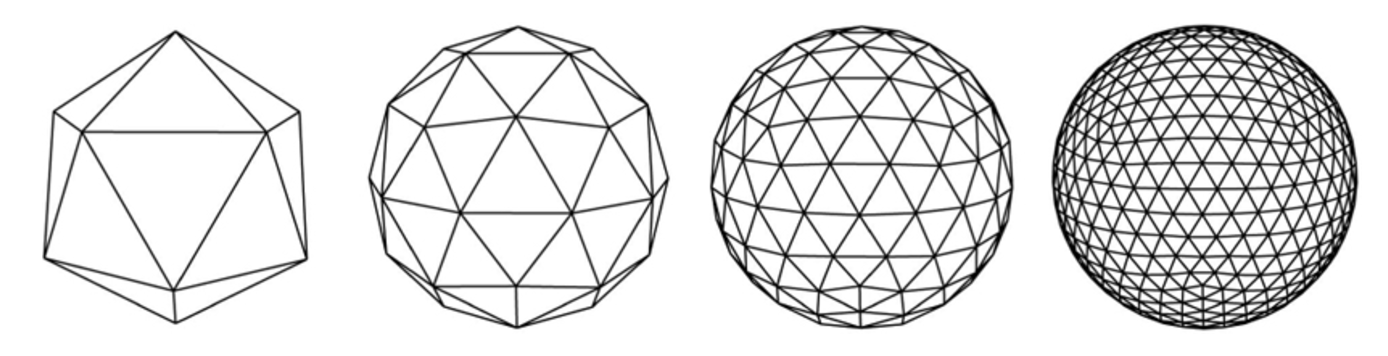
\includegraphics[width=\linewidth]{split_exmpl}
	\caption{Деление граней икосаэдра посредством бисекции}
	\label{split_exmpl}
\end{figure}

На рисунке \ref{phys} представлена схема алгоритма расчета физических параметров слайма.

\begin{figure}[H]
	\centering
	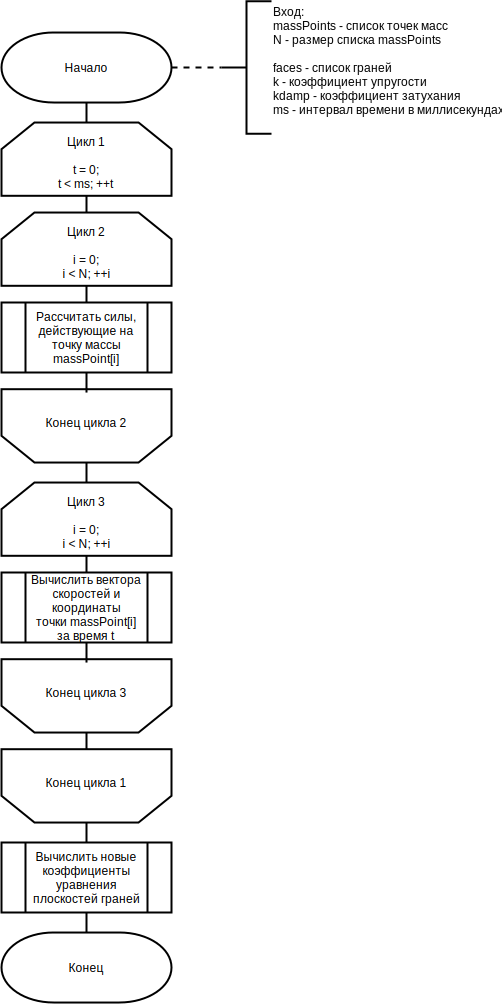
\includegraphics[width=0.6\linewidth]{phys}
	\caption{Схема алгоритма расчета физических параметров слайма}
	\label{phys}
\end{figure}

На каждую точку массы действуют три силы:

\begin{itemize}
	\item сила тяжести;
	\item сила упругости со стороны пружины;
	\item сила затухания со стороны демпфера;
\end{itemize}

Вектор силы тяжести вычисляется по формуле:

\begin{equation}\label{mg}
	F_{\text{тяж}_i} = m_i g,
\end{equation}
где $m_i$ --- масса $i$-ой точки,\\
\text{~~~~~~} $g$ --- вектор ускорения свободного падения, $|g| = 9.81 \frac{\text{Н}}{\text{м}}$.

Сила упругости определяется по закону Гука~\cite{muller}:

\begin{equation}\label{hooke}
	F_{\text{упр}_{ij}} = -k (|x_{ij}| - l_{ij}) \frac{x_{ij}}{|x_{ij}|},
\end{equation}
где $k$ --- жесткость пружины, соединяющей точки масс $i$ и $j$;\\
\text{~~~~~~}$x_{ij}$ --- разница радиус-векторов точек масс $j$ и $i$ соответственно,\\
\text{~~~~~~}$l_{ij}$ --- расстояние между точками масс $i$ и $j$, при котором сила упругости равна нулю.

Затухающая сила вычисляется по формуле~\cite{muller}:

\begin{equation}\label{damp}
	F_{\text{сопр}_{ij}} = -k_d \frac{(v_{ij}; x_{ij})}{(x_{ij}; x_{ij})} \frac{x_{ij}}{|x_{ij}|},
\end{equation}
где $k_d$ --- коэффициент затухания,\\
\text{~~~~~~}$x_{ij}$ --- разница радиус-векторов точек масс $j$ и $i$ соответственно,\\
\text{~~~~~~}$v_{ij}$ --- разница векторов скокростей точек масс $j$ и $i$ соответственно.

В итоге, используя формулы \eqref{mg}, \eqref{hooke} и \eqref{damp}, можно вычислить равнодействующую всех сил, приложенных к $i$-ой точку массы:

\begin{equation}\label{f}
	F_i = F_{\text{тяж}_i} + \sum_{j}^{K_i} (F_{\text{упр}_{ij}} + F_{\text{сопр}_{ij}}),
\end{equation}
где $K_i$ --- количество пружин, которые имеет $i$-ая точка массы.

Из нашей модели, используемой для моделирования слайма, следует, что вся масса объекта распределяется по его поверхности, а не по объему. Из этого следует, что если всем пружинам, отвечающим за упругие взаимодействия между точками, присвоить одинаковые значения коэффициента упругости, то моделирование тела будет не совсем верным по эстетическим соображениям.

Для решения данной проблемы автор работы предлагает представить пружины как совокупности последовательно соединенных элементарных пружин одинаковой длины покоя $d_e$ и коэффициента упругости $k_e$. Тогда количество элементарных пружин будет равно:
\begin{equation}\label{stifn}
	n = \frac{d}{d_e},
\end{equation}
где $d$ --- длина покоя пружины, соединяющей точки масс.

Наконец, коэффициент упругости системы последовательно соединенных пружин будет равен:
\begin{equation}\label{stif}
	k = \frac{k_e}{n} = \frac{k_e d_e}{d},
\end{equation}

Вектор ускорения точки вычисляется по второму закону Ньютона:

\begin{equation}\label{sln}
	a_i = \frac{F_i}{m_i},
\end{equation}
где $m_i$ --- масса $i$-ой точки,\\
\text{~~~~~~}$F_i$ --- равнодействующая всех сил, приложенных к $i$-ой точке.

В соответствии с полученным ускорением, вычисляется вектор скорости $i$-ой точки массы по формуле:

\begin{equation}\label{velocity}
	v_i = v_{0_i} + a_i t,
\end{equation}
где $v_{0_i}$ --- начальная скорость $i$-ой точки,\\
\text{~~~~~~}$t$ --- время, в течение которого изменяется скорость под действием сил, $t = 1~\text{мс}$.

Новые координаты точки вычисляются по формуле:

\begin{equation}\label{new_pos}
	P_i(x, y, z) = P_{0_i}(x_0, y_0, z_0) + v_{0_i} t + a_i t^2,
\end{equation}
где $P_{0_i}(x_0, y_0, z_0)$ --- радиус-вектор начального положения $i$-ой точки в пространстве,\\
\text{~~~~~~}$v_{0_i}$ --- начальная скорость $i$-ой точки,\\
\text{~~~~~~}$a_i$ --- ускорение $i$-ой точки,\\
\text{~~~~~~}$t$ --- время, в течение которого изменяется скорость под действием сил.

\section[Разработка рекурсивного алгоритма обратной трассировки лучей]{Разработка рекурсивного алгоритма\\обратной трассировки лучей}

На рисунке \ref{ray_tracing} приведена схема рекурсивного алгоритма обратной трассировки лучей.

\begin{figure}[H]
	\centering
	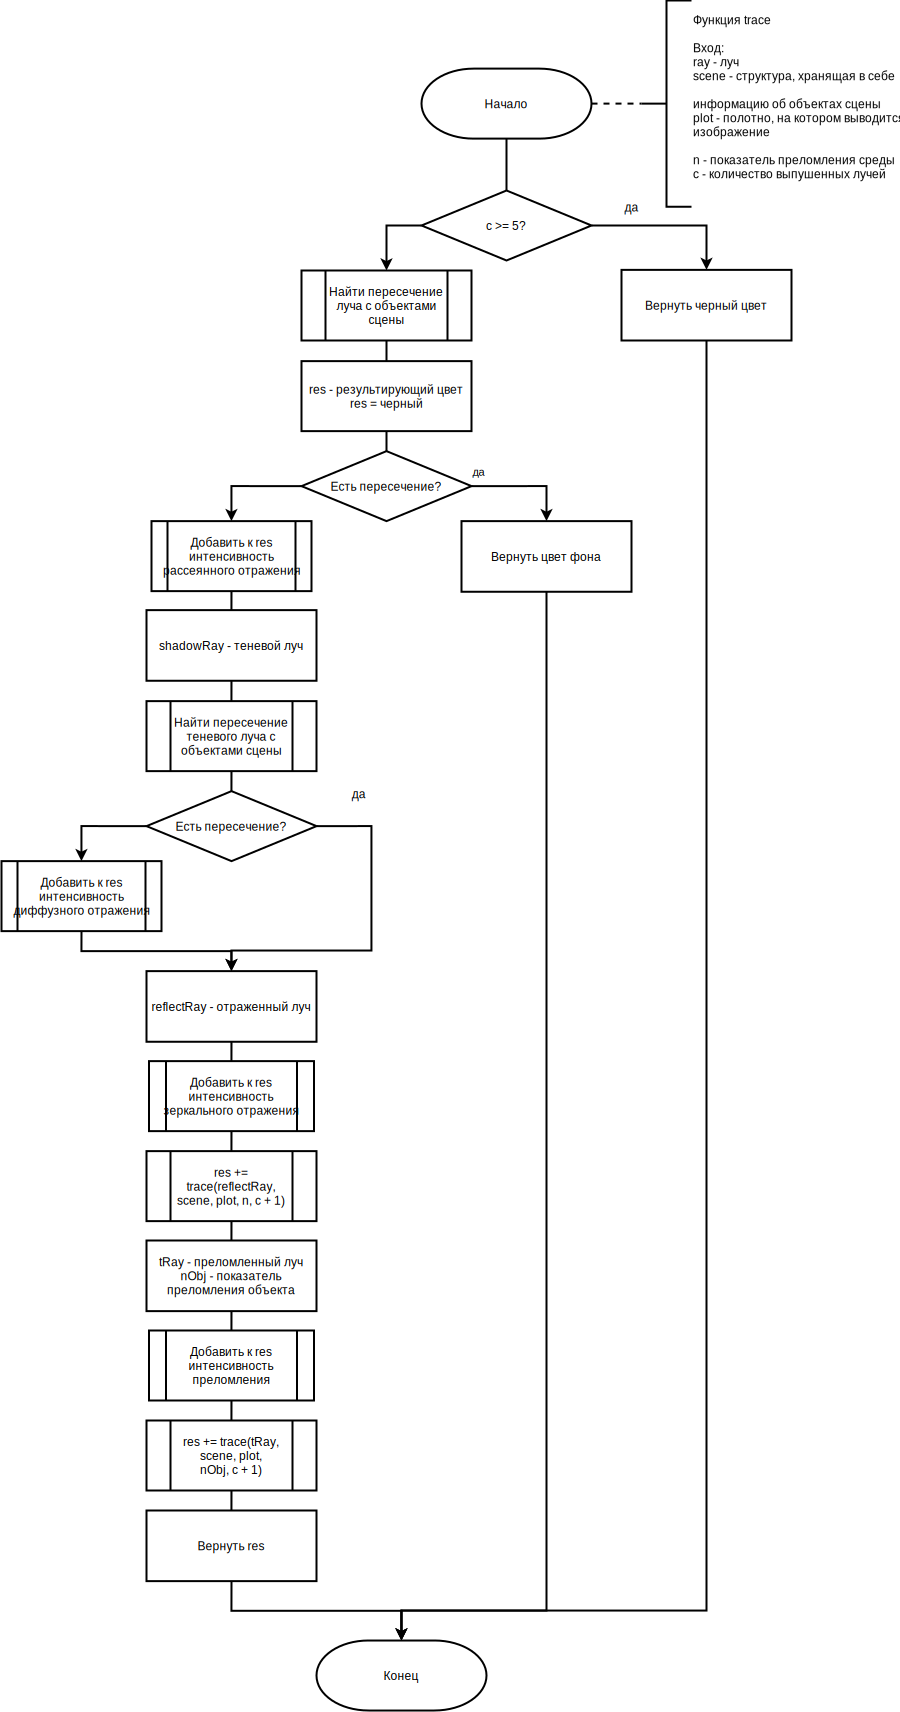
\includegraphics[width=0.8\columnwidth]{ray_tracing}
	\caption{Схема алгоритма обратной трассировки лучей}
	\label{ray_tracing}
\end{figure}

Вектор отраженного от плоской поверхности луча можно найти по формуле~\cite{raytracingen}:

\begin{equation}\label{refl}
	v_r = v - 2(n; v)n,
\end{equation}
где $v$ --- вектор падающего на поверхность луча,\\
\text{~~~~~~}$n$ --- нормаль к поверхности.

Вектор преломленного луча определяется по формуле~\cite{raytracingen}:

\begin{equation}\label{refr}
	v_t = \frac{n_0}{n} v - (\frac{n_0}{n}(N; v) + cos\theta_t)N,
\end{equation}
где $v$ --- вектор падающего на поверхность луча,\\
\text{~~~~~~}$N$ --- нормаль к поверхности,\\
\text{~~~~~~}$n_0$ --- показатель преломления среды, из которой падает луч $v$,\\
\text{~~~~~~}$n$ --- показатель преломления среды, в которую падает луч $v$,\\
\text{~~~~~~}$\theta_t$ --- угол между нормалью $n$ и преломленным лучом.

Угол $\theta_t$ вычисляется по закону Снеллиуса~\cite{raytracingen}:

\begin{equation}\label{snell}
	\theta_t = \frac{n_0sin(\theta)}{n},
\end{equation}
где $\theta$ --- угол между нормалью $N$ и вектором луча $v$.

Встает вопрос о поиске точки пересечения луча с треугольной гранью слайма. Любую точку, лежащую на луче, можно описать следующим выражением:

\begin{equation}\label{ray}
	P(x, y, z) = P_0(x_0, y_0, z_0) + tl(x_l, y_l, z_l),
\end{equation}
где $P_0(x_0, y_0, z_0)$ --- радиус-вектор начальной точки луча,\\
\text{~~~~~~}$l(x_l, y_l, z_l)$ --- вектор направления луча,\\
\text{~~~~~~}$t \in \mathbb{R},$ $t \ge 0$.

Точку пересечения луча с треугольной гранью слайма можно найти с помощью барицентрического теста~\cite{intersection}. Суть данного метода заключается в том, что любую точку пространства можно перевести в барицентрическую систему координат, связанную с треугольником.

Пусть даны треугольная грань с вершинами $v_1$, $v_2$ и $v_3$. Тогда точка пересечения луча, описанного выражением \eqref{ray}, с гранью может быть определена с помощью решения:

\begin{equation}\label{bar}
	\begin{bmatrix}
		t\\
		u\\
		v
	\end{bmatrix}
	= \frac{1}{(S; E_1)}
	\begin{bmatrix}
		(Q; E_2)\\
		(S; T)\\
		(Q; l)
	\end{bmatrix},
\end{equation}
где $(u, v)$ --- барицентрические координаты точки пересечения,\\
\text{~~~~~~}$E_1 = v_2 - v_1$,\\
\text{~~~~~~}$E_2 = v_3 - v_1$,\\
\text{~~~~~~}$T = P_0 - v_1$,\\
\text{~~~~~~}$S = [l; E_2]$,\\
\text{~~~~~~}$Q = [T; E_1]$.

Если $u \in [0, 1]$, $v \in [0, 1]$ и $t \ge 0$, то найденная точка пересечения лежит внутри треугольника.

Для ускорения работы реализации алгоритма обратной трассировки лучей используется сферическая объемлющая оболочка слайма. Следовательно, встает вопрос об определении признака пересечения полупрямой с поверхностью шара.

Пусть луч задан выражением \eqref{ray}, а оболочка имеет центр в точке $C(x_c, y_c, z_c)$ и радиус $R$, то есть описывается уравнением:

\begin{equation}\label{sphere}
	(x - x_c)^2 + (y - y_c)^2 + (z - z_c)^2 = R^2.
\end{equation}

Тогда полупрямая пересекает сферу, если имеет хотя бы одно неотрицательное решение следующее уравнение:
\begin{equation}\label{spheq1}
	(x_0 + tx_l - x_c)^2 + (y_0 + ty_l - y_c)^2 + (z_0 + tz_l - z_c)^2 = R^2.
\end{equation}

После раскрытия скобок и приведения подобных слагаемых получаем выражение:

\begin{equation}\label{spheq2}
	at^2 + bt + c = 0,
\end{equation}
где $a = x_l^2 + y_l^2 + z_l^2$,\\
\text{~~~~~~}$b = 2(x_l(x_0 - x_c) + y_l(y_0 - y_c) + z_l(z_0 - z_c))$,\\
\text{~~~~~~}$c = (x_0 - x_c)^2 + (y_0 - y_c)^2 + (z_0 - z_c) ^ 2 - R^2$.

Полученное квадратное уравнение имеет хотя бы одно решение, если его дискриминант неотрицателен:
\begin{equation}\label{sphd}
	D = b^2 - 4ac.
\end{equation}

Тогда корни вычисляются по формуле:
\begin{equation}
	t_{1,2} = \frac{-b \pm \sqrt{D}}{2a}.
\end{equation}

Если хотя бы одно найденное решение неотрицательно, то луч пересекает сферу.

\section[Разработка алгоритма захвата точки слайма пользователем]{Разработка алгоритма захвата точки\\слайма пользователем}

Программа моделирования слайма должна обеспечивать управление объектом. В частности, пользователь должен иметь возможность растягивать и вдавливать тело.

На рисунке \ref{grabbing} приведена схема алгоритма захвата точки слайма пользователем.

\begin{figure}[H]
	\centering
	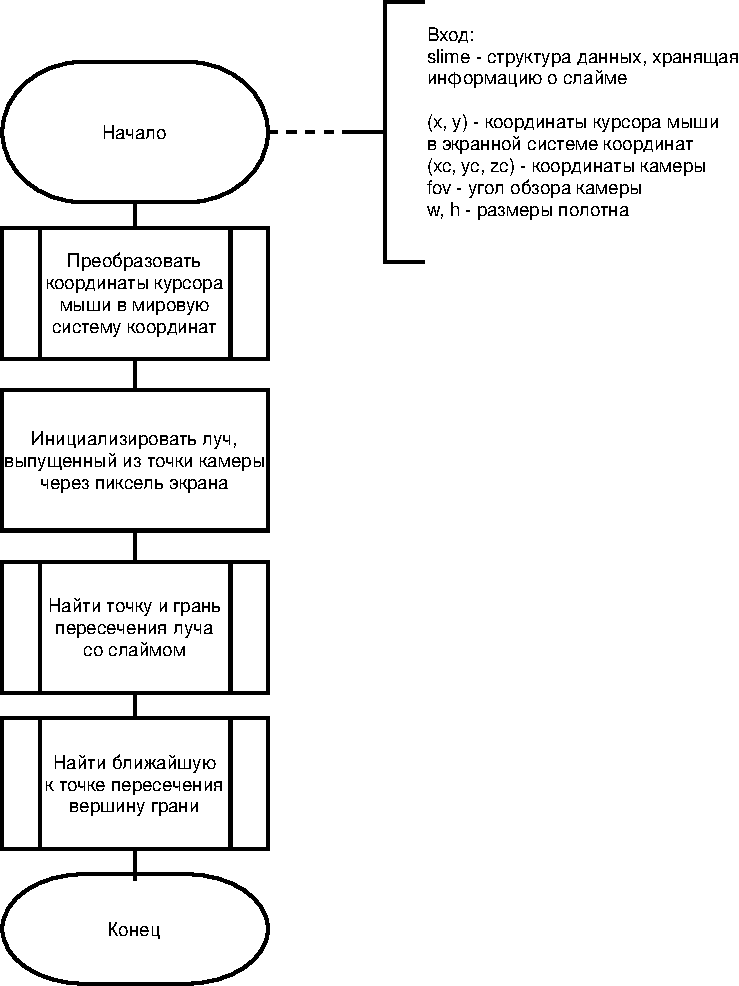
\includegraphics[width=0.6\linewidth]{grabbing}
	\caption{Схема алгоритма захвата точки слайма пользователем}
	\label{grabbing}
\end{figure}

\section*{Вывод}
В данном разделе были описаны существующие алгоритмы, необходимые для разработки программного обеспечения и разработаны методы для данной работы.

\clearpage
